% PSI Beamer presentation: the LESTO case ladder, one slide per case.
% Every number on a slide comes from a repository file (run/<case>/readme.md,
% notes.md, dictionaries, out logs, expect*.json, verification.json, the
% tracked records of 023 and 024) or from a run made for this deck
% (runs/runs.json; figures and their inputs: figure_sources.json).
% The PSI theme files and assets are those of presentations/m10-project-review.
\PassOptionsToPackage{table}{xcolor}
\documentclass[aspectratio=169,10pt]{beamer}
\usetheme{PSI}
\usepackage{amsmath,amssymb}
\usepackage{fancyvrb}
\usefonttheme{professionalfonts}
\ifXeTeX
  \setsansfont{Liberation Sans}
  \setmonofont{Liberation Mono}
\fi
\ifLuaTeX
  \setsansfont{Liberation Sans}
  \setmonofont{Liberation Mono}
\fi
\graphicspath{{figures/}{psi-assets/}{./}}
\setbeameroption{hide notes}
\setbeamerfont{title}{size=\fontsize{25}{29}\selectfont,series=\bfseries}
\setbeamerfont{subtitle}{size=\fontsize{14}{18}\selectfont,series=\mdseries}
\setbeamerfont{section page}{size=\fontsize{26}{31}\selectfont,series=\bfseries}
\renewcommand{\PSIfootername}{PSI \enspace | \enspace LESTO Task 3.4 \enspace | \enspace The case ladder}
\renewcommand{\PSIfootdate}{15.10.2026}

\title{The LESTO case ladder}
\subtitle{From a laminar pipe to the benchmark studies,\\one change per case}
\author{Jan Kren}
\institute{LESTO Task 3.4 \enspace | \enspace Villigen PSI}
\date{15 October 2026}
\psititlestyle{blue}

\setbeamercolor{codebox}{fg=PSIblack,bg=PSIlightgray!22}
\setbeamercolor{changebox}{fg=PSIblack,bg=PSIblue!8}
\newcommand{\PbI}{\ensuremath{\mathrm{PbI}_2}}
\newcommand{\BiI}{\ensuremath{\mathrm{BiI}_3}}
% based-on line, the one change, checks and run line of a case slide
\newcommand{\basedon}[2]{{\small\color{PSIgray}#1\enspace|\enspace #2}\par\vspace{0.25em}}
\newcommand{\change}[1]{\begin{beamercolorbox}[sep=0.35em,wd=\linewidth]{changebox}\small\raggedright\textbf{#1}\end{beamercolorbox}\vspace{0.3em}}
\newcommand{\runline}[1]{\par\vspace{0.3em}{\raggedright\small\textbf{Run:} #1\par}}
\newcommand{\figsrc}[1]{\par\vspace{0.1em}{\raggedright\small\color{PSIgray}#1\par}}
\newcommand{\casefig}[1]{\centering\includegraphics[width=\linewidth,height=0.56\textheight,keepaspectratio]{#1}}
\setlength{\leftmargini}{1.0em}
\AtBeginEnvironment{itemize}{\small\setlength{\itemsep}{1pt}}
\fvset{fontsize=\small,xleftmargin=0pt}
% written by make_figures.py
\newcommand{\VAReightdiff}{max $|$PbI$_2-$tracer$|$/max = 0}
\newcommand{\VARtwelveclosure}{$|$closure$|$/released 1.7e-16}
\newcommand{\VAReightT}{257}
\newcommand{\VARnineT}{559}
\newcommand{\VARtenT}{502}
\newcommand{\VARelevenT}{399}

\tikzset{
  lad/.style={draw=#1,fill=#1!10,rounded corners=1.5pt,minimum width=1.0cm,minimum height=0.62cm,inner sep=1pt,font=\small\bfseries},
  bk/.style={->,>=stealth,line width=0.6pt,draw=PSIgray}}
\colorlet{cCarrier}{PSIblue}
\colorlet{cSpecies}{PSIpurple}
\colorlet{cExchange}{PSIred}
\colorlet{cBench}{PSIgreen!55!black}

\begin{document}

% 01 title ---------------------------------------------------------------
{\setbeamertemplate{footline}{}\setbeamertemplate{headline}{}
\begin{frame}[plain]
  \titlepage
  \note{The case ladder in run/ of the LESTO repository: 24 cases, each adding one thing to the case it is based on. Cases 001 to 011 are Bojan Ničeno's: the pipe, the helium carrier and the species transport. Cases 012 to 024 are mine: the gas and condensate exchange, step by step, and the three benchmark studies. Every number on the slides comes from a file of the repository or from a run made for this deck on 15 October 2026.}
\end{frame}}

% 02 overview -------------------------------------------------------------
\begin{frame}[t]{The ladder: 24 cases, one change each}
  \centering
  \begin{tikzpicture}[x=1.26cm,y=1.22cm]
    \foreach \n [count=\i from 0] in {001,002,003,004,005,006,007}
      \node[lad=cCarrier] (n\n) at (\i,0) {\n};
    \foreach \n [count=\i from 7] in {008,009,010,011}
      \node[lad=cSpecies] (n\n) at (\i,0) {\n};
    \foreach \a/\b in {001/002,002/003,003/004,004/005,005/006,006/007,007/008,008/009,009/010,010/011}
      \draw[bk] (n\a) -- (n\b);
    \node[lad=cExchange] (n012) at (10,-1.25) {012};
    \node[lad=cExchange] (n013) at (9,-1.25) {013};
    \node[lad=cExchange] (n014) at (8,-1.25) {014};
    \node[lad=cExchange] (n016) at (7,-1.25) {016};
    \node[lad=cExchange] (n017) at (6,-1.25) {017};
    \node[lad=cExchange] (n015) at (9,-2.5) {015};
    \node[lad=cExchange] (n018) at (8,-2.5) {018};
    \node[lad=cExchange] (n019) at (7,-2.5) {019};
    \node[lad=cExchange] (n020) at (7,-3.75) {020};
    \node[lad=cExchange] (n021) at (6,-2.5) {021};
    \node[lad=cBench] (n022) at (10,-2.5) {022};
    \node[lad=cBench] (n023) at (5,-1.25) {023};
    \node[lad=cBench] (n024) at (5,-2.5) {024};
    \draw[bk] (n011) -- (n012);
    \foreach \a/\b in {012/013,013/014,014/016,016/017,017/023,013/015,014/018,018/019,019/020,019/021,021/024,012/022}
      \draw[bk] (n\a) -- (n\b);
    \draw[bk,dashed] (n017) -- (n024);
    % legend
    \node[anchor=north west,align=left,font=\small,text width=5.0cm] at (-0.45,-0.85) {%
      \textcolor{cCarrier}{\rule{7pt}{7pt}} carrier flow 001--007\\
      \textcolor{cSpecies}{\rule{7pt}{7pt}} species transport 008--011\\
      \hspace*{1.0em}{\color{PSIgray}cases by Bojan Ničeno}\\[0.3em]
      \textcolor{cExchange}{\rule{7pt}{7pt}} gas/condensate exchange 012--021\\
      \textcolor{cBench}{\rule{7pt}{7pt}} benchmarks 022--024\\
      \hspace*{1.0em}{\color{PSIgray}cases by Jan Kren}\\[0.3em]
      {\color{PSIgray}arrow: ``based on''; dashed: carrier}\\
      {\color{PSIgray}technique of 017 used by 024}};
  \end{tikzpicture}
  \note{The arrows are the based-on links of the readmes. The trunk runs from the laminar pipe of 001 to the coupled species sources of 011, then turns to the wall laws: the temperature model in 012, the Hertz-Knudsen-Schrage law in 013, the synthetic channel in 014. Side branches end in cases no later case builds on: 015 and 020 need the optional GEMS3K build, 022 is the paper-mode benchmark of the temperature model. 023 and 024 are the two experimental benchmark studies; 024 is based on 021 and uses the physical-carrier technique of 017. New cases go on top, from 025.}
\end{frame}

% 03 how to read ----------------------------------------------------------
\begin{frame}[t]{Every case: the same four parts}
  \begin{columns}[T,onlytextwidth]
    \begin{column}{0.48\textwidth}
      \psiheading{readme.md of each case}
      \begin{itemize}
        \item ``This case is based on case N''
        \item the changed dictionary lines
        \item the numbers to check
        \item how to run it
      \end{itemize}
      \vspace{0.4em}
      \psiheading{001--011 (Bojan Ničeno)}
      {\small Run in place: \texttt{gmsh}, \texttt{simpleFoam} or \texttt{rhoSimpleFoam}; 008--011 read the mesh of 001 and the carrier of 007 at 261 through links.\par}
    \end{column}
    \begin{column}{0.48\textwidth}
      \psiheading{012--024 (Jan Kren)}
      \begin{itemize}
        \item \texttt{./Allrun}: the default check into \texttt{work/}
        \item ends with one line PASS, FAIL or NOTRUN
        \item compared with \texttt{out\_excerpt} or \texttt{expect.json}
        \item \texttt{./Allrun-ladder 012-024}: one line per case
      \end{itemize}
      \vspace{0.4em}
      \psiheading{Figures in this deck}
      {\small Real outputs: tracked logs and records, or runs made for this deck in a scratch copy of \texttt{run/} on 3 cores (\texttt{runs/runs.json}).\par}
    \end{column}
  \end{columns}
  \note{The run/readme.md is the index. No Allrun writes a tracked file; everything goes into the git-ignored work directory of the case. Without an external input, such as the restricted bismuth thermodynamic tables, a case prints NOTRUN and the sweep continues. For this deck the cases were copied into a scratch directory and run there, with OpenFOAM v2412 and the M10e solver binary, sha256 16fd804e, pinned to cores 4, 5 and 11.}
\end{frame}

% ==========================================================================
\psisectionstyle{blue}
\section{\texorpdfstring{Carrier flow 001--007\\[0.25em]{\Large\mdseries cases by Bojan Ničeno}}{Carrier flow 001--007}}

% 001 ---------------------------------------------------------------------
\begin{frame}[t,fragile]{001 first-pipe-flow-simpleFoam}
  \begin{columns}[T,onlytextwidth]
    \begin{column}{0.53\textwidth}
      \basedon{The first case}{Bojan Ničeno}
      \change{Laminar helium pipe, gmsh mesh, steady \texttt{simpleFoam}}
      \begin{beamercolorbox}[sep=0.3em,wd=\linewidth]{codebox}
\begin{Verbatim}
INLET  uniform (0.095 0 0); // m/s
nu     1.6265e-4;   // m2/s, He
\end{Verbatim}
      \end{beamercolorbox}
      \begin{itemize}
        \item R = 2.4 mm, L = 0.69 m, 228,960 hexahedra
        \item \texttt{checkMesh}: Mesh OK
        \item converged in 235 SIMPLE iterations
      \end{itemize}
    \end{column}
    \begin{column}{0.45\textwidth}
      \casefig{c001}
      \figsrc{Mesh of \texttt{pipe.msh}; \texttt{001/out}}
      \runline{\texttt{gmsh}, \texttt{gmshToFoam}, \texttt{simpleFoam}}
    \end{column}
  \end{columns}
  \note{The geometry is that of Francesco's T-Flows LESTO cases, vapour-pressure model, with the internal wall renamed WALL. Helium at rho 0.166 kg per cubic metre and mu 2.70e-5 Pa s; outlet pressure zero, no-slip wall. The cross-section is the INLET patch of the converted mesh, 540 faces: an O-grid core with a refined wall layer. The SIMPLE iterations are pseudo-time, not a transient.}
\end{frame}

% 002 ---------------------------------------------------------------------
\begin{frame}[t,fragile]{002 parabolic-inlet}
  \begin{columns}[T,onlytextwidth]
    \begin{column}{0.53\textwidth}
      \basedon{Based on case 001}{Bojan Ničeno}
      \change{Parabolic inlet profile, \texttt{codedFixedValue} in \texttt{0/U}}
      \begin{beamercolorbox}[sep=0.3em,wd=\linewidth]{codebox}
\begin{Verbatim}
const scalar R    = 0.0024;
const scalar Umax = 0.19;
Ux = Umax*(1.0 - r2/(R*R));
\end{Verbatim}
      \end{beamercolorbox}
      \begin{itemize}
        \item bulk velocity about 0.095 m/s: same flow rate as 001
        \item internal field still uniform 0.095 m/s
        \item converged in 388 iterations (001: 235)
      \end{itemize}
    \end{column}
    \begin{column}{0.45\textwidth}
      \casefig{c002}
      \figsrc{\texttt{0/U}; \texttt{001/out}, \texttt{002/out}}
      \runline{as 001, \texttt{simpleFoam > out}}
    \end{column}
  \end{columns}
  \note{Only 0/U changed. OpenFOAM compiles the coded boundary condition at run time into dynamicCode/parabolicInlet. The parabolic inlet meets a uniform initial field, which costs iterations: 388 instead of 235. Case 003 removes that mismatch.}
\end{frame}

% 003 ---------------------------------------------------------------------
\begin{frame}[t,fragile]{003 parabolic-initialization}
  \begin{columns}[T,onlytextwidth]
    \begin{column}{0.53\textwidth}
      \basedon{Based on case 002}{Bojan Ničeno}
      \change{Parabolic initial field with \texttt{setExprFields}}
      \begin{beamercolorbox}[sep=0.3em,wd=\linewidth]{codebox}
\begin{Verbatim}
U { field U; expression #{ vector(
  0.19*(1.0 - (sqr(pos().y())
   + sqr(pos().z()))/sqr(0.0024)),
  0, 0) #}; }
\end{Verbatim}
      \end{beamercolorbox}
      \begin{itemize}
        \item inlet boundary condition unchanged from 002
        \item converged in 222 iterations (002: 388)
      \end{itemize}
    \end{column}
    \begin{column}{0.45\textwidth}
      \casefig{c003}
      \figsrc{\texttt{002/out}, \texttt{003/out}}
      \runline{\texttt{setExprFields; simpleFoam}}
    \end{column}
  \end{columns}
  \note{system/setExprFieldsDict writes the same parabola into the internal field, so the initial condition is consistent with the inlet. The first Ux residual of 003 is already below 1e-2, and the iteration count drops from 388 to 222.}
\end{frame}

% 004 ---------------------------------------------------------------------
\begin{frame}[t,fragile]{004 energy-with-rhoSimpleFoam}
  \begin{columns}[T,onlytextwidth]
    \begin{column}{0.53\textwidth}
      \basedon{Based on case 003}{Bojan Ničeno}
      \change{\texttt{rhoSimpleFoam} and the energy equation}
      \begin{beamercolorbox}[sep=0.3em,wd=\linewidth]{codebox}
\begin{Verbatim}
type heRhoThermo;
equationOfState rhoConst;
Cp 5193; Pr 0.916;  // T = 300 K
\end{Verbatim}
      \end{beamercolorbox}
      \begin{itemize}
        \item p in Pa: 101325 at the outlet
        \item criteria (\texttt{fvSolution}): U 1e-4, p 1e-3, e 1e-3
        \item converged in 154 iterations
      \end{itemize}
    \end{column}
    \begin{column}{0.45\textwidth}
      \casefig{c004}
      \figsrc{\texttt{004/out}; dotted: the criteria}
      \runline{\texttt{setExprFields; rhoSimpleFoam}}
    \end{column}
  \end{columns}
  \note{The physics stays that of 003: constant density 0.166, inlet and wall at 300 K. The readme lists the pressure criterion as 1e-4; the tracked system/fvSolution has p 1e-3, which is what the figure draws. The energy residual is the last to fall below its criterion, at iteration 154.}
\end{frame}

% 005 ---------------------------------------------------------------------
\begin{frame}[t,fragile]{005 varying-wall-temperature}
  \begin{columns}[T,onlytextwidth]
    \begin{column}{0.53\textwidth}
      \basedon{Based on case 004}{Bojan Ničeno}
      \change{Linear wall temperature, 400 K to 300 K}
      \begin{beamercolorbox}[sep=0.3em,wd=\linewidth]{codebox}
\begin{Verbatim}
WALL { type codedFixedValue;
  T = 400.0 - 100.0*x/0.69; }
INLET  uniform 400;
\end{Verbatim}
      \end{beamercolorbox}
      \begin{itemize}
        \item internal T initialised with the same ramp
        \item energy residual far lower than in 004
        \item converged in 154 iterations
      \end{itemize}
    \end{column}
    \begin{column}{0.45\textwidth}
      \casefig{c005}
      \figsrc{\texttt{0.orig/T}; \texttt{004/out}, \texttt{005/out}}
      \runline{\texttt{setExprFields; rhoSimpleFoam}}
    \end{column}
  \end{columns}
  \note{Modified files: 0.orig/T and system/setExprFieldsDict. Because the initial temperature already matches the wall ramp, the energy equation starts close to its solution: its first residual is about 1e-5 against 1 in case 004. The iteration count, 154, is set by the other equations.}
\end{frame}

% 006 ---------------------------------------------------------------------
\begin{frame}[t,fragile]{006 variable-density}
  \begin{columns}[T,onlytextwidth]
    \begin{column}{0.53\textwidth}
      \basedon{Based on case 005}{Bojan Ničeno}
      \change{Ideal-gas density from local p and T}
      \begin{beamercolorbox}[sep=0.3em,wd=\linewidth]{codebox}
\begin{Verbatim}
type            hePsiThermo;
equationOfState perfectGas;
molWeight       4.0026;
\end{Verbatim}
      \end{beamercolorbox}
      \begin{itemize}
        \item was \texttt{heRhoThermo + rhoConst}
        \item viscosity, Cp and Pr still constant
        \item converged in 230 iterations (005: 154)
      \end{itemize}
    \end{column}
    \begin{column}{0.45\textwidth}
      \casefig{c006}
      \figsrc{\texttt{006/out}; dashed: \texttt{005/out}}
      \runline{\texttt{setExprFields; rhoSimpleFoam}}
    \end{column}
  \end{columns}
  \note{Only constant/thermophysicalProperties changed. With density coupled to temperature the pressure residual oscillates in the first 30 iterations and the run needs 230 iterations instead of 154.}
\end{frame}

% 007 ---------------------------------------------------------------------
\begin{frame}[t,fragile]{007 variable-properties-high-temperature}
  \begin{columns}[T,onlytextwidth]
    \begin{column}{0.53\textwidth}
      \basedon{Based on case 006}{Bojan Ničeno}
      \change{Sutherland transport, wall 1000 K to 300 K}
      \begin{beamercolorbox}[sep=0.3em,wd=\linewidth]{codebox}
\begin{Verbatim}
transport sutherland;
As 1.4683e-06;  Ts 83.40;
T_wall = 1000.0 - 700.0*x/0.69;
\end{Verbatim}
      \end{beamercolorbox}
      \begin{itemize}
        \item writes \texttt{mu} and \texttt{kappa} (coded function object)
        \item converged in 261 iterations: the carrier at 261
        \item 28 mL/min, T and U overwritten: development carrier
      \end{itemize}
    \end{column}
    \begin{column}{0.45\textwidth}
      \casefig{c007}
      \figsrc{\texttt{007/261}, foamToVTK}
      \runline{\texttt{setExprFields; rhoSimpleFoam}}
    \end{column}
  \end{columns}
  \note{The saved carrier at time 261 is what 008 to 013 read through links: U, p, T, rho and phi. Its temperature equals the wall ramp at every radius, and the velocity has no radial component: its T and U were overwritten in commit 3ce3791, which is why the notes of 012 and 013 call it a development carrier, plan section 8, risk 10. Its consistency is max of T minus p W over R rho, relative, 0.0030. The physical carriers come in 017.}
\end{frame}

% ==========================================================================
\psisectionstyle{purple}
\section{\texorpdfstring{Species transport 008--011\\[0.25em]{\Large\mdseries cases by Bojan Ničeno}}{Species transport 008--011}}

% 008 ---------------------------------------------------------------------
\begin{frame}[t,fragile]{008 one-species-transport-rhoFixedFlowFoam}
  \begin{columns}[T,onlytextwidth]
    \begin{column}{0.53\textwidth}
      \basedon{Based on case 007}{Bojan Ničeno}
      \change{\texttt{rhoFixedFlowFoam}: gaseous species on the frozen carrier}
      \begin{beamercolorbox}[sep=0.3em,wd=\linewidth]{codebox}
\begin{Verbatim}
species ( PbI2_g tracer );
PbI2_g { state gas; D 1.0e-5; }
tracer { state gas; D 1e-5; }
\end{Verbatim}
      \end{beamercolorbox}
      \begin{itemize}
        \item no momentum, pressure or energy solve
        \item same D, inlet and initial field: identical $Y$
        \item run for this deck to 1 s: \VAReightdiff
      \end{itemize}
    \end{column}
    \begin{column}{0.45\textwidth}
      \casefig{c008}
      \figsrc{Deck run: 1 s, 3 ranks, \VAReightT{} s}
      \runline{\texttt{rhoFixedFlowFoam > out}}
    \end{column}
  \end{columns}
  \note{The species equation is ddt of rho Y plus div of phi Y minus laplacian of rho D Y equals zero, for every species in the run-time list. Inlet mass fraction 1e-6, time step 4 ms. The two species must stay identical; this checks the multi-species loop before species-specific diffusivities. The deck run stopped at 1 s instead of the case's 16 s, to keep it below a few minutes.}
\end{frame}

% 009 ---------------------------------------------------------------------
\begin{frame}[t,fragile]{009 variable-diffusivity}
  \begin{columns}[T,onlytextwidth]
    \begin{column}{0.53\textwidth}
      \basedon{Based on case 008}{Bojan Ničeno}
      \change{PbI$_2$--He diffusivity from the carrier T and p}
      \begin{beamercolorbox}[sep=0.3em,wd=\linewidth]{codebox}
\begin{Verbatim}
PbI2_g { diffusivityModel PbI2He; }
tracer { diffusivityModel constant;
         D 1e-5; }
\end{Verbatim}
      \end{beamercolorbox}
      \begin{itemize}
        \item D evaluated once at start-up, then fixed
        \item \texttt{D\_PbI2\_g}: 3.089e-5 to 2.536e-4 m$^2$/s
        \item tracer uncoupled, solved after PbI$_2$
      \end{itemize}
    \end{column}
    \begin{column}{0.45\textwidth}
      \casefig{c009}
      \figsrc{Deck run: 1 s, 3 ranks, \VARnineT{} s}
      \runline{\texttt{rhoFixedFlowFoam > out}}
    \end{column}
  \end{columns}
  \note{The diffusivity range is the start-up line of the tracked out_excerpt. The correlation pressure is in atmospheres; the carrier is at 1 atm. On the hot side the PbI2 diffusivity is up to 25 times the tracer's, so the PbI2 front is more smeared than the tracer front. The PbI2 residual history is expected to reproduce that of the single-species case.}
\end{frame}

% 010 ---------------------------------------------------------------------
\begin{frame}[t,fragile]{010 handles-solid-species}
  \begin{columns}[T,onlytextwidth]
    \begin{column}{0.53\textwidth}
      \basedon{Based on case 009}{Bojan Ničeno}
      \change{A solid species and a mock thermochemistry call}
      \begin{beamercolorbox}[sep=0.3em,wd=\linewidth]{codebox}
\begin{Verbatim}
PbI2_s { state solid; }
S = S0*(Thot - T)/(Thot - Tcold);
S0 1e-6; Thot 1000; Tcold 300;
\end{Verbatim}
      \end{beamercolorbox}
      \begin{itemize}
        \item solid: only $\partial_t(\rho Y) = S$, \texttt{diagonal} solver
        \item source kept in the 15,264 wall-adjacent cells
        \item no coupling: max $Y$ grows linearly in time
      \end{itemize}
    \end{column}
    \begin{column}{0.45\textwidth}
      \casefig{c010}
      \figsrc{Tracked \texttt{010/out\_excerpt}, 16 s run}
      \runline{\texttt{rhoFixedFlowFoam > out}}
    \end{column}
  \end{columns}
  \note{evaluateThermochemistry receives T, p, the species list and the local values, and returns one source per species: the interface a GEMS call will use later. S0 is in kg per cubic metre and second. The solid grows linearly in time, independently of the gas, which is the point of the mock: the gas equations are unchanged from 009. The figure is the tracked excerpt of the original 16 s run with OpenFOAM v2606: the maximum mass fraction of PbI2_s grows by 2.93e-8 per 4 ms step to 1.17e-4. Today's solver carries the coupled mock source of 011 in the same routine, so case 010 cannot be rerun as it was; the deck run of 010 behaved like 011 and is not shown.}
\end{frame}

% 011 ---------------------------------------------------------------------
\begin{frame}[t,fragile]{011 coupled-species-sources}
  \begin{columns}[T,onlytextwidth]
    \begin{column}{0.53\textwidth}
      \basedon{Based on case 010}{Bojan Ničeno}
      \change{Gas PbI$_2$ deposits as solid: equal and opposite sources}
      \begin{beamercolorbox}[sep=0.3em,wd=\linewidth]{codebox}
\begin{Verbatim}
rate = K*max(Y_PbI2_g, 0)
  *max((Thot-T)/(Thot-Tcold), 0);
K 1.0;  // kg/(m3 s), WALL cells
\end{Verbatim}
      \end{beamercolorbox}
      \begin{itemize}
        \item gas sink implicit; solid takes what the gas lost
        \item excerpt: net thermochemistry source 0 kg/s
        \item full mass ledger not yet (comes in 012)
      \end{itemize}
    \end{column}
    \begin{column}{0.45\textwidth}
      \casefig{c011}
      \figsrc{Deck run: 1 s, 3 ranks, \VARelevenT{} s}
      \runline{\texttt{rhoFixedFlowFoam > out}}
    \end{column}
  \end{columns}
  \note{The tracer is dropped. Every step prints the integrated source of PbI2_g and PbI2_s and their sum; in the tracked excerpt the sum is exactly 0 kg per second while the individual rates grow from 4.4e-18 kg per second. The solid sits where gas has arrived and the wall is cooler than 1000 K.}
\end{frame}

% ==========================================================================
\psisectionstyle{red}
\section{\texorpdfstring{Gas/condensate exchange 012--021\\[0.25em]{\Large\mdseries cases by Jan Kren}}{Gas/condensate exchange 012--021}}

% 012 ---------------------------------------------------------------------
\begin{frame}[t,fragile]{012 temperature-model}
  \begin{columns}[T,onlytextwidth]
    \begin{column}{0.53\textwidth}
      \basedon{Based on case 011}{Jan Kren}
      \change{Wall law of Lobresco et al.\ (2026), Eq.~5, a release boat and a mass ledger}
      \begin{beamercolorbox}[sep=0.3em,wd=\linewidth]{codebox}
\begin{Verbatim}
model temperature;
temperatureCoeffs {A 220;
  k 8e-3; Tdep 680;}
boat {mode release; amount 3.16e-5;
      duration 6;}    // mol, s
\end{Verbatim}
      \end{beamercolorbox}
      \begin{itemize}
        \item 15,264 wall elements, $v_d$ = 0.0124421 m/s
        \item closure step 5: $-1.36\times10^{-16}$; 6 s: 1.8e-14
        \item deck run: max \VARtwelveclosure
      \end{itemize}
    \end{column}
    \begin{column}{0.45\textwidth}
      \casefig{c012}
      \figsrc{Deck run: \texttt{steps 100}, 1 core, 260 s}
      \runline{\texttt{./Allrun}: excerpt PASS}
    \end{column}
  \end{columns}
  \note{The wall flux is minus rho v_d times the positive part of one minus exp of minus k times Tdep minus T, times Y; irreversible. Every kilogram is booked: gas, wall, released, transport, clamped and solver defect, and the closure is their difference. The default Allrun reproduced the 123 lines of out_excerpt exactly in the deck run. Over the whole 6 s release the closure stays at 1.8e-14 and the released amount equals n0 M to 2e-16, criterion M2.2g.}
\end{frame}

% 013 ---------------------------------------------------------------------
\begin{frame}[t,fragile]{013 hks-inventory}
  \begin{columns}[T,onlytextwidth]
    \begin{column}{0.53\textwidth}
      \basedon{Based on case 012}{Jan Kren}
      \change{Hertz--Knudsen--Schrage law at the wall and in an evaporating boat}
      \begin{beamercolorbox}[sep=0.3em,wd=\linewidth]{codebox}
\begin{Verbatim}
model HKS; equilibrium table;
phases ("PbI2(cr)" "PbI2(l)");
mode inventory; amount 4.84e-6;
\end{Verbatim}
      \end{beamercolorbox}
      \begin{itemize}
        \item $p_{eq}$: lower of crystal and liquid, cross at 683 K
        \item $\lambda\,\Delta t$ = 1000 to 1900: stiff, implicit
        \item closure $-1.9\times10^{-16}$; deck run: boat 4.84 $\rightarrow$ 4.34 $\mu$mol in 0.1 s
      \end{itemize}
    \end{column}
    \begin{column}{0.45\textwidth}
      \casefig{c013}
      \figsrc{$p_{eq}$ table; deck run, 100 steps}
      \runline{\texttt{./Allrun}: excerpt PASS}
    \end{column}
  \end{columns}
  \note{The boat holds 4.84e-6 mol, 2.23 mg, the inventory of experiment T106_6, and is removed at 6 s. The vapour-pressure table is from the NASA-9 records of Gurvich 1991. The final tolerance of the PbI2 solve went from 1e-12 to 1e-14: with 1e-12 the solver defect grew to 2e-8 of the inventory over 16 s. The wall stays empty near the boat because the walls there are far above the saturation temperature. Over 100 steps the boat lost 0.50 micromol to the gas.}
\end{frame}

% 014 ---------------------------------------------------------------------
\begin{frame}[t,fragile]{014 hks-channel}
  \begin{columns}[T,onlytextwidth]
    \begin{column}{0.53\textwidth}
      \basedon{Based on case 013}{Jan Kren}
      \change{The synthetic plane channel, 1000 K to 350 K: axial profiles and $T_{dep}$}
      \begin{beamercolorbox}[sep=0.3em,wd=\linewidth]{codebox}
\begin{Verbatim}
// 0.1 m x 4.8 mm, 100 x 24 cells
Tin 1000; Tout 350;
massFlux 0.01743;
onset {fraction .01;}
\end{Verbatim}
      \end{beamercolorbox}
      \begin{itemize}
        \item 1 \% onset 561.164 K, 5.89 K below plug flow (gate 10 K)
        \item 99.5 \% of the release on the wall at 3 s
        \item closures 2.5e-16 (pair), 4.05e-16 (Pb, I)
      \end{itemize}
    \end{column}
    \begin{column}{0.45\textwidth}
      \casefig{c014}
      \figsrc{Deck run, wall profile at 3 s}
      \runline{\texttt{./Allrun}, 10 s: PASS 9/9}
    \end{column}
  \end{columns}
  \note{The channel is made by blockMesh and filled by the test helper makeCarrier with plug flow and a linear temperature; every later development case uses it. The release is 2.80e-11 mol PbI2 over 2 s into a box of 40 cells. The 1 percent onset is the paper's definition of T_dep, on the condensate. Its PbI2 ledger and profiles are byte-identical to the PbI2 pair of case 018, checked in the deck run as well.}
\end{frame}

% 015 ---------------------------------------------------------------------
\begin{frame}[t,fragile]{015 hks-gems-local}
  \begin{columns}[T,onlytextwidth]
    \begin{column}{0.53\textwidth}
      \basedon{Based on case 013}{Jan Kren}
      \change{$p_{eq}$ from GEMS3K for every wall element and boat cell, every step}
      \begin{beamercolorbox}[sep=0.3em,wd=\linewidth]{codebox}
\begin{Verbatim}
HKSCoeffs {equilibrium GEMS;}
GEMSCoeffs {mode local;
  minTemperature 500;
  maxLog10Deviation 0.01;}
\end{Verbatim}
      \end{beamercolorbox}
      \begin{itemize}
        \item 576 to 720 calls per step, 0 failures
        \item GEMS and table agree to 1e-5 to 1e-4 decades
        \item balance and closure those of 013 to round-off
      \end{itemize}
    \end{column}
    \begin{column}{0.45\textwidth}
      \casefig{c015}
      \figsrc{Tracked \texttt{out\_excerpt}, 5 steps}
      \runline{needs the bridge build: not run}
    \end{column}
  \end{columns}
  \note{The table stays as a guard: below 500 K, below a mole fraction of 1e-6, outside the system's grid, for a failed call or a result more than 0.01 decades off the table, the element takes the table. Step 1 makes no call: 4356 wall faces are below 500 K and no other element has gas. For this ideal PbI2-He gas the case shows the coupling, not a new physical result. The whole excerpt is compared only with the bridge that wrote it, md5 fb67103e; this workstation's solver has no bridge, so the case would print NOTRUN.}
\end{frame}

% 016 ---------------------------------------------------------------------
\begin{frame}[t,fragile]{016 hks-channel-halfcell}
  \begin{columns}[T,onlytextwidth]
    \begin{column}{0.53\textwidth}
      \basedon{Based on case 014}{Jan Kren}
      \change{Half-cell diffusion resistance in series with the HKS law}
      \begin{beamercolorbox}[sep=0.3em,wd=\linewidth]{codebox}
\begin{Verbatim}
interface {patches (WALL);
           wallResistance halfCell;}
\end{Verbatim}
      \end{beamercolorbox}
      \begin{itemize}
        \item conductance 63.7--107 $\rightarrow$ 0.98--0.99 m/s
        \item onset moves 5 mK: 561.1645 $\rightarrow$ 561.1593 K
        \item peak 7.4 \% lower, one bin downstream; L1 6.6 \%
      \end{itemize}
    \end{column}
    \begin{column}{0.45\textwidth}
      \casefig{c016}
      \figsrc{Deck runs 014 and 016, at 3 s}
      \runline{\texttt{./Allrun}, 10 s: PASS 9/9}
    \end{column}
  \end{columns}
  \note{On this mesh the half-cell conductance D over dy/2 is 1 m per second, 64 to 107 times smaller than the kinetic conductance, so it controls the uptake. Where the deposit starts, the gas reaches the wall by diffusion either way, so the onset moves by only 5 mK, far inside one 1 mm bin of 6.5 K. halfCell is the wall law of every physical run: 017, 023 and 024.}
\end{frame}

% 016, continued: Damkoehler sweep --------------------------------------
\begin{frame}[t,fragile]{016 hks-channel-halfcell: Damk\"ohler sweep}
  \begin{columns}[T,onlytextwidth]
    \begin{column}{0.53\textwidth}
      \basedon{Case 016 unchanged except $\alpha$}{Jan Kren}
      \change{Accommodation $\alpha$ over six decades: Da from $10^{-3}$ to $2\times10^{3}$}
      \begin{beamercolorbox}[sep=0.3em,wd=\linewidth]{codebox}
\begin{Verbatim}
// PbI2_g pair and HKSCoeffs:
accommodation 1e-6 ... 1;
// 13 runs, 5 refined
\end{Verbatim}
      \end{beamercolorbox}
      \begin{itemize}
        \item $\hat J=\mathrm{Da}$ for Da $\le$ 0.01; plateau $\pi^2/4$ above 300
        \item deposited 0.3 $\rightarrow$ 99.5 \%; onset stays at 561 K
        \item $\alpha=0.1$: profile 1.4 \%; $\alpha=0.01$: 14 \%
      \end{itemize}
    \end{column}
    \begin{column}{0.45\textwidth}
      \centering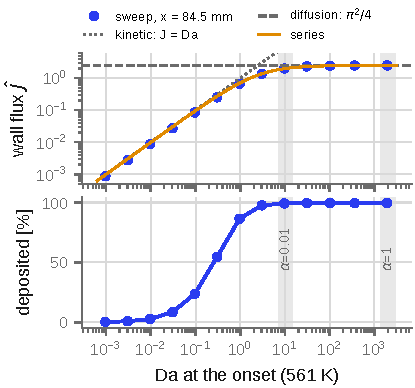
\includegraphics[width=\linewidth,height=0.5\textheight,keepaspectratio]{c016b}
      \figsrc{Record \texttt{manuscript/data/damkohler}}
      \runline{\texttt{./Allrun-damkohler}, a few minutes}
    \end{column}
  \end{columns}
  \note{The wall Damkoehler number compares the kinetic conductance of the HKS law with diffusion over the channel half-height. Varying only the accommodation coefficient moves it over six decades. Below 0.1 the wall flux equals Da: the wall sees the bulk gas and the kinetics decide. Above about 300 it reaches pi squared over four, the diffusion limit of plug flow between absorbing plates, and between the two it follows the series-resistance curve. The deposit then moves 11 mm upstream and its width halves, but the onset temperature does not move, because saturation sets it. The grey bands are the Damkoehler numbers of the production tube cases: alpha 1 and 0.1 lie on the diffusion plateau, alpha 0.01 at its edge. This is the Damkoehler figure of Sec. 4.2 of the manuscript; refinement changes every number by less than 0.11 percent.}
\end{frame}

% 017 ---------------------------------------------------------------------
\begin{frame}[t,fragile]{017 physical-carrier}
  \begin{columns}[T,onlytextwidth]
    \begin{column}{0.53\textwidth}
      \basedon{Based on case 016}{Jan Kren}
      \change{The physical carrier of Lobresco T106\_6: 106 mL/min, measured wall T}
      \begin{beamercolorbox}[sep=0.3em,wd=\linewidth]{codebox}
\begin{Verbatim}
// wedge 5 deg, R 2.4 mm, 212 x 48
massFlowRate 4.3817e-09; // kg/s
interfaceTemperature wall;
\end{Verbatim}
      \end{beamercolorbox}
      \begin{itemize}
        \item carrier audit PASS, cell flux defect 1.2e-17
        \item $T_{dep}$ 839.09 K: +25.73 K against 814 K
        \item peak 4 cm upstream; closure 2.1e-16
      \end{itemize}
    \end{column}
    \begin{column}{0.45\textwidth}
      \casefig{c017}
      \figsrc{Record \texttt{023/cases/coarse/T106\_6}}
      \runline{\texttt{./Allrun}, about 8 min}
    \end{column}
  \end{columns}
  \note{The carrier is computed with rhoSimpleFoam, expanding and laminar, projected to an exactly divergence-free flux, audited, and frozen. The boat of 013 returns at the digitised arrow, x = 0.13 m, with the wedge share of the inventory, 6.72e-8 mol. The inlet is zero-total-flux for the gas. Not represented: the boat obstruction, the end of the experiment and the non-dilute gas next to the boat. The figure is the tracked final profile of case 023's coarse T106_6, which 017's Allrun reproduces byte for byte with the M10e solver; the case was not rerun for the deck.}
\end{frame}

% 018 ---------------------------------------------------------------------
\begin{frame}[t,fragile]{018 pbi2-bii3-channel}
  \begin{columns}[T,onlytextwidth]
    \begin{column}{0.53\textwidth}
      \basedon{Based on case 014}{Jan Kren}
      \change{A second, independent pair: BiI$_3$ from the same boat}
      \begin{beamercolorbox}[sep=0.3em,wd=\linewidth]{codebox}
\begin{Verbatim}
BiI3_g {condensed BiI3_s;
  HKS {accommodation 1; ...}
  vapourPressure {phases
    ("BiI3(cr)" "BiI3(l)");}}
\end{Verbatim}
      \end{beamercolorbox}
      \begin{itemize}
        \item onsets: PbI$_2$ 561.164 K, BiI$_3$ 449.979 K
        \item plug flow: 567.057 K and 450.383 K
        \item closures Pb 4.05e-16, Bi 4.56e-16, I 4.37e-16
      \end{itemize}
    \end{column}
    \begin{column}{0.45\textwidth}
      \casefig{c018}
      \figsrc{Deck run, wall profiles at 3 s}
      \runline{\texttt{./Allrun}: PASS 8/8}
    \end{column}
  \end{columns}
  \note{The source ratio follows the inferred PbI2 and BiI3 deposits of Liu et al. 2025, LBE-I_SS_II. The two pairs do not interact, so the PbI2 results are those of 014 byte for byte, criterion M10a.1; the deck run confirmed that. The BiI3 table is made from restricted Bi thermodynamic records and is not redistributed; without it the case prints NOTRUN. A qualification case, not the paper's geometry.}
\end{frame}

% 019 ---------------------------------------------------------------------
\begin{frame}[t,fragile]{019 pbbi-gas-speciation}
  \begin{columns}[T,onlytextwidth]
    \begin{column}{0.53\textwidth}
      \basedon{Based on case 018}{Jan Kren}
      \change{Nine gases in homogeneous equilibrium, every cell and step}
      \begin{beamercolorbox}[sep=0.3em,wd=\linewidth]{codebox}
\begin{Verbatim}
respeciation {engine kernel;
  species (Pb_g PbI_g PbI2_g Bi_g
    Bi2_g BiI_g BiI3_g I_g I2_g);
  minTemperature 350;}
\end{Verbatim}
      \end{beamercolorbox}
      \begin{itemize}
        \item inlet 1173 K: onsets 559.778 K and 444.563 K
        \item vs 018 at 1173 K: 0.0000844 \% and 0.1332 \%
        \item element closures 4.3--5.0e-16
      \end{itemize}
    \end{column}
    \begin{column}{0.45\textwidth}
      \casefig{c019}
      \figsrc{Deck run, wall profiles at 3 s}
      \runline{\texttt{./Allrun}, 457 s: PASS 7/7}
    \end{column}
  \end{columns}
  \note{The exact kernel uses tabulated formation constants. The inlet is raised to 1173 K, the LBE furnace, so that there is something to re-speciate. The percentages are the 1 cm deposit L1 differences from the independent pairs of 018 run at the same inlet; 2 ms against 1 ms gives 0.0331 and 0.0575 percent. Numerical results under provisional inputs: synthetic ramp, common diffusivity, prescribed release.}
\end{frame}

% 020 ---------------------------------------------------------------------
\begin{frame}[t,fragile]{020 pbbi-gems-speciation}
  \begin{columns}[T,onlytextwidth]
    \begin{column}{0.53\textwidth}
      \basedon{Based on case 019}{Jan Kren}
      \change{Re-speciation by GEMS3K: modes \texttt{frozen} and \texttt{local}}
      \begin{beamercolorbox}[sep=0.3em,wd=\linewidth]{codebox}
\begin{Verbatim}
respeciation {engine GEMS;
  GEMS {mode frozen;
    carrier "He(g)";
    minMoleFraction 1e-12;}}
\end{Verbatim}
      \end{beamercolorbox}
      \begin{itemize}
        \item L1 frozen vs kernel: 1.03e-10, 1.06e-7
        \item local vs frozen: 0; closure 6.7e-16
        \item 132.2 $\mu$s per local call (5,814,420 calls)
      \end{itemize}
    \end{column}
    \begin{column}{0.45\textwidth}
      \casefig{c020}
      \figsrc{\texttt{020/qualification.json}}
      \runline{needs the bridge build: not run}
    \end{column}
  \end{columns}
  \note{Mode frozen caches the formation constants at the frozen cell temperatures and pressures, then uses the exact kernel. Mode local calls GEMS3K per cell and step, warm started, with guards and the kernel as refinement and fallback. For an ideal gas both must reproduce 019, and they do. The figure shows why the refinement is needed: the raw interior-point result is off by up to about half a decade at mole fractions near 1e-10; decades above 1e-3 are guarded and never called.}
\end{frame}

% 021 ---------------------------------------------------------------------
\begin{frame}[t,fragile]{021 lbe-metal-vapour}
  \begin{columns}[T,onlytextwidth]
    \begin{column}{0.53\textwidth}
      \basedon{Based on case 019}{Jan Kren}
      \change{Metal vapour, shared condensates and reactive wall channels}
      \begin{beamercolorbox}[sep=0.3em,wd=\linewidth]{codebox}
\begin{Verbatim}
BiI {reactant BiI_g;
  condensed Bi_s; reversible no;
  stoichiometry {BiI_g -3;
    Bi_s 2; BiI3_g 1;}}
\end{Verbatim}
      \end{beamercolorbox}
      \begin{itemize}
        \item five onsets within 3.89 K of plug flow
        \item half step changes none of them
        \item closures 3.7--4.6e-16
      \end{itemize}
    \end{column}
    \begin{column}{0.45\textwidth}
      \casefig{c021}
      \figsrc{Deck run, profiles at 1.2 s}
      \runline{\texttt{./Allrun}, 45 s: PASS 8/8}
    \end{column}
  \end{columns}
  \note{The Q2 source releases monatomic Pb, Bi and I; the metal vapour is 1 percent of the ideal-LBE saturation pressure at 1173 K. Pb_g condenses on Pb_s; Bi_g and Bi2_g on one shared Bi_s; BiI_g reacts irreversibly at the wall to 2 Bi_s and BiI3_g. Onsets, solver against fractional plug flow: Pb(l) 919.93 against 921, Bi(l) 882.89 against 885, PbI2(cr) 533.12 against 537, Bi(cr) 541.35 against 544, BiI3(cr) 450.82 against 451 K. The carrier is the plug-flow limit, 200 by 2 cells with D = 0, read at 1.2 s while the source is active.}
\end{frame}

% ==========================================================================
\psisectionstyle{green}
\section{\texorpdfstring{Benchmarks 022--024\\[0.25em]{\Large\mdseries cases by Jan Kren}}{Benchmarks 022--024}}

% 022 ---------------------------------------------------------------------
\begin{frame}[t,fragile]{022 paper-temperature-model}
  \begin{columns}[T,onlytextwidth]
    \begin{column}{0.53\textwidth}
      \basedon{Based on case 012}{Jan Kren}
      \change{Paper mode: code-to-code with T-Flows, Figs.~8--10 and Table 2}
      \begin{beamercolorbox}[sep=0.3em,wd=\linewidth]{codebox}
\begin{Verbatim}
// setFrozenCarrier: rho 1,
//   1.67e-6 m3/s (100 mL/min)
interface {layer distance;
           distance 1e-4;}
amount 3.16e-5; duration 15;
\end{Verbatim}
      \end{beamercolorbox}
      \begin{itemize}
        \item gas plateau at 16 s: +0.5 \% against Fig.~9
        \item solid onset $-25.9$ mm; T-Flows set: $-0.9$ mm
        \item Table 2: all ten lines within max(2 K, $\Delta T_{bin}$)
      \end{itemize}
    \end{column}
    \begin{column}{0.45\textwidth}
      \casefig{c022}
      \figsrc{Wall table; onsets: readme, notes}
      \runline{\texttt{./Allrun}, 38 s: excerpt PASS}
    \end{column}
  \end{columns}
  \note{The layer is the T-Flows layer of cell centres within 0.1 mm of the wall, 30528 cells, A_I over V_I 8533.7 per metre. The plateau, n0 over the bulk velocity, agrees. The deposit starts where the wall table crosses the input Tdep of 680 K, at 0.476 m, 2.6 cm upstream of the published onset at 0.502 m; the T-Flows parameter set, Tdep 638.15 K, A 150, k 0.02, distance 2.4e-4, puts it at 0.5011 m. Which set produced the paper's figures is a question for the authors. The full 30 s case takes 2 to 3 hours on 16 ranks and was not rerun.}
\end{frame}

% 023 ---------------------------------------------------------------------
\begin{frame}[t,fragile]{023 lobresco2026}
  \begin{columns}[T,onlytextwidth]
    \begin{column}{0.53\textwidth}
      \basedon{Based on case 017}{Jan Kren}
      \change{All five PbI$_2$ experiments of Lobresco et al.\ (2026), two meshes}
      \begin{beamercolorbox}[sep=0.3em,wd=\linewidth]{codebox}
\begin{Verbatim}
// T106_6 T106_60 T106_300
// T5_60 T540_60
prod:   318 x 72 = 22,896 cells
coarse: 212 x 48 (case 017)
\end{Verbatim}
      \end{beamercolorbox}
      \begin{itemize}
        \item $\Delta T_{dep}$: +26, +19, +16, $-11$, $-14$ K
        \item RMS 18 K; the paper's two models: 35 K
        \item coarse = prod within 0.3 K; closure 3.3e-16
      \end{itemize}
    \end{column}
    \begin{column}{0.45\textwidth}
      \casefig{c023}
      \figsrc{Records \texttt{cases/prod}; data CC BY 4.0}
      \runline{\texttt{./Allrun prod T106\_6 ...}}
    \end{column}
  \end{columns}
  \note{No parameter is adjusted to these data. The rule is the paper's: 1 percent of the peak of the deposit, from the inlet, on the measured wall curve, minus the measurement of Table 2. At 5 mL per minute vapour diffuses upstream and deposits near the cold inlet; the table uses the main deposit downstream of the boat. Computed peaks lie 1 to 4 cm upstream of the measured ones. This is Sec. 6.3, Table V and Fig. 5 of the manuscript.}
\end{frame}

% 024 ---------------------------------------------------------------------
\begin{frame}[t,fragile]{024 liu2025}
  \begin{columns}[T,onlytextwidth]
    \begin{column}{0.53\textwidth}
      \basedon{Based on case 021 (+ carrier of 017)}{Jan Kren}
      \change{Liu et al.\ (2025): Pb--Bi--I chemistry on physical carriers}
      \begin{beamercolorbox}[sep=0.3em,wd=\linewidth]{codebox}
\begin{Verbatim}
interfaceTemperature wall;
wallResistance halfCell;
// Q1; Q2 at 0.1, 1, 10 % saturation
\end{Verbatim}
      \end{beamercolorbox}
      \begin{itemize}
        \item 576 x 72, limitedLinear: 19 PASS
        \item PbI$_2$ peak 36 cm / 366.5 $^\circ$C vs 368 $\pm$ 18 $^\circ$C
        \item mesh 1.98 \% (one case); correctors $\le$ 0.021 \%
      \end{itemize}
    \end{column}
    \begin{column}{0.45\textwidth}
      \casefig{c024}
      \figsrc{\texttt{production\_576x72\_limitedLinear}}
      \runline{\texttt{./Allrun full} (6 h per case)}
    \end{column}
  \end{columns}
  \note{Three configurations on 1.25 m columns of steel and silica, 5-degree wedges, measured wall temperatures, Q1 the deposited amount over three hours, Q2 LBE metal vapour with two BiI datasets, 2 ms steps, 60 s. Provisional numerical work: the release history, the flow reference conditions and several coordinates are assumptions. The mesh number is the iodine profile change of the shifted-BiI steel case between 41,472 and 93,312 cells with the production scheme; no formal GCI, the apparent orders are inconsistent. Every element closure stays at or below 8.63e-16. The next slide has the checks made after the review. manuscript/check_results.py recomputes these numbers from the saved profiles.}
\end{frame}

% 024, continued: checks of the production runs ------------------------
\begin{frame}[t,fragile]{024 liu2025: sensitivities, mesh and GEMS3K}
  \begin{columns}[T,onlytextwidth]
    \begin{column}{0.53\textwidth}
      \basedon{Production cases of 024}{Jan Kren}
      \change{The checks behind the production runs, made after the review}
      \begin{beamercolorbox}[sep=0.3em,wd=\linewidth]{codebox}
\begin{Verbatim}
production_sensitivities/   // 8 runs
scheme_mesh_study/upwind_L4/ // 4 runs
\end{Verbatim}
      \end{beamercolorbox}
      \begin{itemize}
        \item limitedLinear: $\alpha$ $\le$ 5.14 \%, $D$ 1.07--16.65 \%
        \item 41,472 $\rightarrow$ 93,312 cells, upwind: 2.13--7.30 \%
        \item GEMS3K in every cell: profiles within 2.1e-4
      \end{itemize}
    \end{column}
    \begin{column}{0.45\textwidth}
      \centering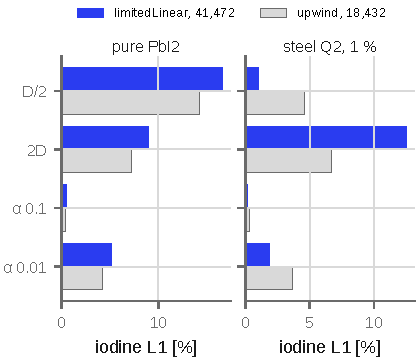
\includegraphics[width=\linewidth,height=0.5\textheight,keepaspectratio]{c024b}
      \figsrc{Record \texttt{024/production\_sensitivities}}
      \runline{\texttt{make\_cases.py}; 17--28 h per case}
    \end{column}
  \end{columns}
  \note{Sensitivities: the diffusivity and accommodation variations of two baselines repeated with the production scheme on 41,472 cells. Accommodation still matters far less than diffusivity, except that in steel halving D changes the profile by only 1.07 percent, because the BiI3 profile, which carries most of the iodine, barely moves; doubling D gives 12.53 percent. Totals change by at most 0.02 percent and the BiI3 share by at most 0.03 points. Mesh: upwind runs of four cases on 93,312 cells change the profiles by 2.13 to 7.30 percent, so the 1.98 percent of the one bounded-scheme case does not bound the others. Correctors: eight instead of three changes the four checked cases by at most 0.021 percent, the shifted-BiI case by 1e-7 percent. GEMS3K: standard-state data in every cell change the profiles by at most 2.1e-4; local mode, 5.1e8 calls without a failure, is bitwise identical to frozen, because its result only starts the kernel solve.}
\end{frame}

% closing -----------------------------------------------------------------
\begin{frame}[t]{What the ladder demonstrates}
  \begin{columns}[T,onlytextwidth]
    \begin{column}{0.52\textwidth}
      \psiheading{One change per case, each checked}
      \begin{itemize}
        \item carrier: pipe to Sutherland helium (001--007)
        \item transport: frozen carrier, species list, coupled sources (008--011)
        \item exchange: every ledger closes at round-off
        \item onsets within 3.89 K of plug flow (021)
        \item wall law: kinetic and diffusion limits (016 sweep)
        \item experiments: $T_{dep}$ RMS 18 K (023)
      \end{itemize}
    \end{column}
    \begin{column}{0.44\textwidth}
      \psiheading{Where it is used}
      \begin{itemize}
        \item methods paper: 016 sweep, 023, 024
        \item deliverable D38: the case ladder of its availability section
        \item \texttt{./Allrun-ladder 012-024}: regression of every check
      \end{itemize}
      \vspace{0.4em}
      \begin{block}{Deck runs, 15.10.2026}
        \small PASS: 012--014, 016, 018, 019, 021, 022. To 1 s: 008, 009, 011. The rest: tracked logs and records.
      \end{block}
    \end{column}
  \end{columns}
  \note{The ladder makes every capability of rhoFixedFlowFoam reproducible from a short readme: what changed, what to check, how to run. Cases 001 to 011 are Bojan Ničeno's groundwork; 012 to 024 add the exchange laws, the chemistry and the benchmark studies. The manuscript's prepare_results.py reads 023 and 024 directly. In this deck every default check that could run on this workstation passed; 015 and 020 need the GEMS3K bridge, 017, 023 and 024 take minutes to hours and are shown from their tracked records.}
\end{frame}

\end{document}
